\subsection{Lancer l'acquisition de données}
\label{start}
\begin{enumerate}
    \item Sur l'interface d'accueil (voir figure~\ref{fig:accueil}), cliquer sur \textit{Camera}.
    \item Sélectionner le \textit{Binning} voulu: 1~=~image plus précise, acquisition plus lente. 4~=~image moins précise, acquisition plus rapide.
    \item Définir l'\textit{Exposure} voulu: valeur plus grande~=~plus de signal détecté par la caméra, acquisition plus lente. Toujours choisir une valeur de 80~ms ou plus.
    \item Cliquer sur X pour fermer la fenêtre.
    \item Cliquer sur \textit{Stop} (bouton rouge).
    \item Cliquer sur \textit{Start Experim.}.
\end{enumerate}
L'acquisition prend un certain temps, dépendamment de la grosseur de l'échantillon et des paramètres de scan choisis. Un cerveau complet de souris peut prendre jusqu'à 10~heures. Pour évaluer le temps d'acquisition: $$dur\acute{e}e~de~l'acquisition = nb~de~slices \cdot nb~de~width~tiles \cdot nb~de~height~tiles \cdot temps~d'exposition$$ Les trois premiers paramètres se retrouvent dans \textit{CFG Experiment}. Le dernier paramètre se retrouve dans \textit{Camera} à \textit{Exposure}.
\\ \\
De plus, il se peut que l'erreur montrée à la figure~\ref{fig:sauce} se produise. Normalement, le problème se règle par lui-même. Cependant, si la fenêtre demeure affichée plus de 15 secondes, il faut éteindre le contrôleur du \textit{sutter ROE-200} (voir figure~\ref{fig:sutter}), attendre quelques secondes et le rallumer.
%
\begin{figure}[H]
%
\begin{minipage}{0.45\textwidth}
\centering
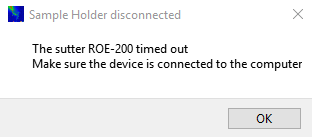
\includegraphics[width=7cm]{sauce.PNG}
\caption{Message d'erreur du \textit{sutter}}
\label{fig:sauce}
\end{minipage}
%
\hfill
%
\begin{minipage}{0.45\linewidth}
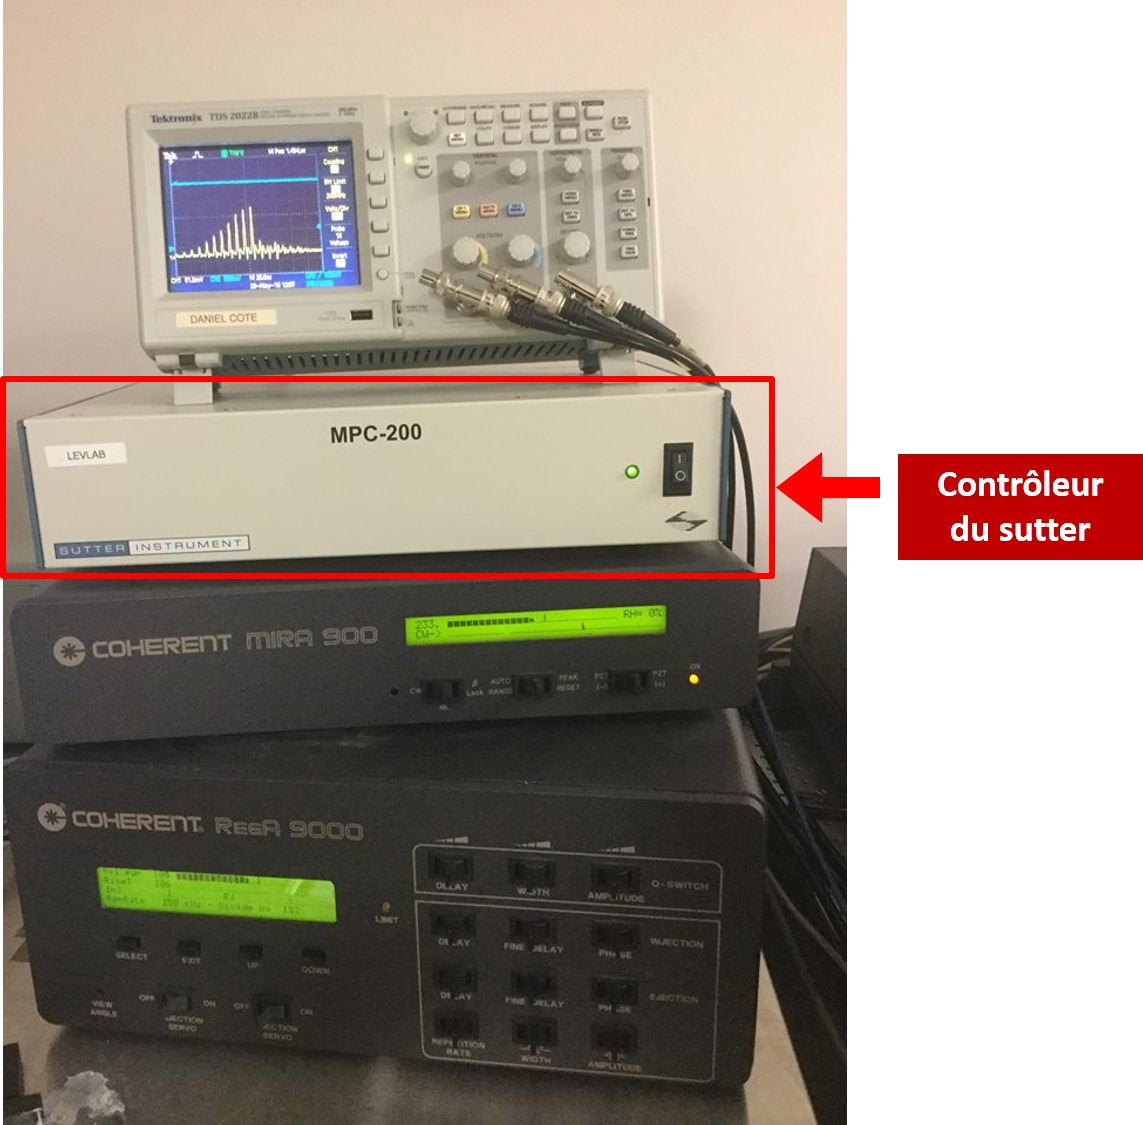
\includegraphics[width=7cm]{sutter.png}
\caption{Contrôleur du \textit{sutter}}
\label{fig:sutter}
\end{minipage}
%
\end{figure}